\documentclass[crop,tikz]{standalone}

\usetikzlibrary{
	chains
}

\begin{document}

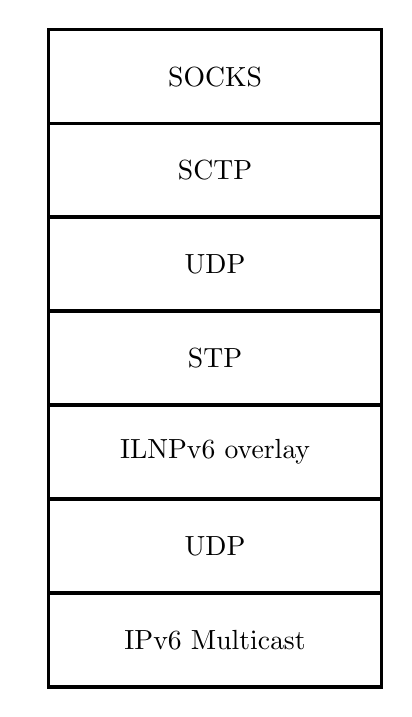
\begin{tikzpicture}[
	node distance = -0.5mm and 0mm,
	start chain = going below,
	layer/.style args = {#1}{
		rectangle, draw, very thick,
		 on chain,
		text width=4cm, align=center,
		minimum height=12mm,
		label=left:#1
	}
]
	\node [layer] {SOCKS};
	\node [layer] {SCTP};
	\node [layer] {UDP};
	\node [layer] {STP};
	\node [layer] {ILNPv6 overlay};
	\node [layer] {UDP};
	\node [layer] {IPv6 Multicast};
\end{tikzpicture}

\end{document}
